\documentclass[a4paper]{article}

\usepackage[utf8]{inputenc}
\usepackage[T1]{fontenc}
\usepackage{graphicx}
\usepackage{hyperref}
\usepackage{amsmath}
\usepackage{amssymb}
\usepackage{mathenv}
\usepackage{multirow}
\usepackage{fullpage}

\DeclareMathAlphabet{\itbf}{OML}{cmm}{b}{it}

% numérotation au sein de chaque section (du style "2.1")
\numberwithin{equation}{section}

% commandes perso
\newcommand{\R}{\mathbb{R}}
\newcommand{\N}{\mathbb{N}}
\newcommand{\C}{\mathcal{C}}
\newcommand{\Ccinf}{\mathcal{C}_c^{\infty}}
\newtheorem{definition}{Definition}

\title{Consistency of Fanbeam Projections of a Translating Object Along an Arc of a Circle}
\author{}
\date{}

\begin{document}

\maketitle

\begin{abstract}
This note aims at extending the results of~\cite{clackdoyle2015consistency} to the case of a translating object.
\end{abstract}

\section{Introduction}

\section{Theory} 
\label{sec:theory}

\subsection{Problem under consideration}
\label{sub:problem_under_consideration}

Let us begin with some notations and definitions. We will consider an object in $\R^2$ to be imaged by a fanbeam source that follows an arc of circle with center $O$ and radius $R_0$ (see Figure~\ref{fig:notations}, left). The object will be identified with its density function $x \mapsto \mu(x) \in \Ccinf$.
\begin{figure}[!ht]
	\centering
	\begin{tabular}{cc}
	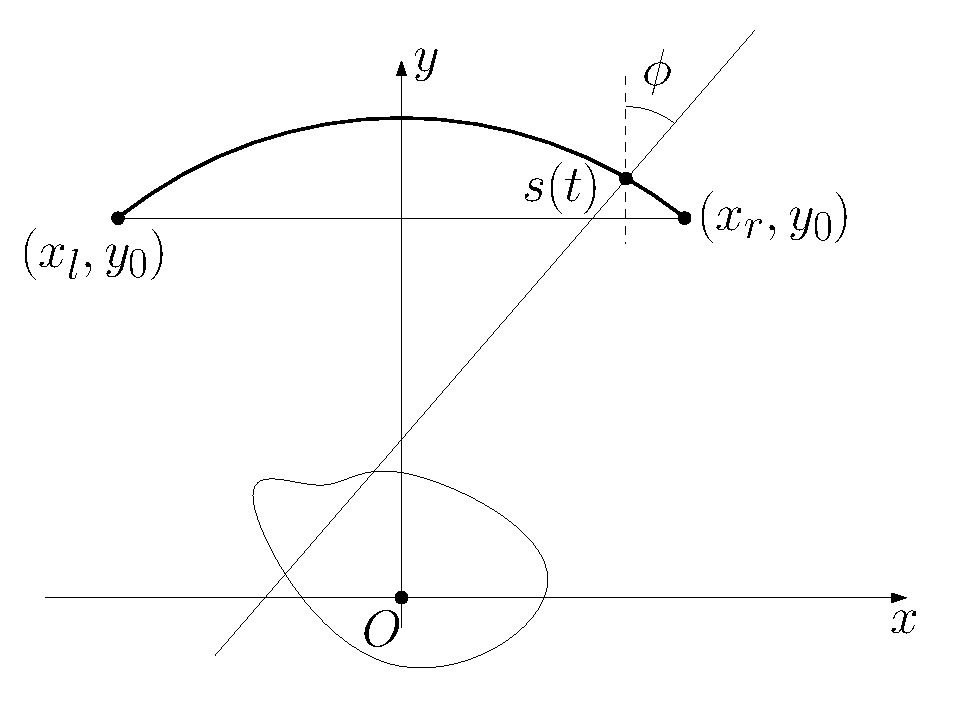
\includegraphics[width=8cm]{figs/frame_scanner_still.eps} &
	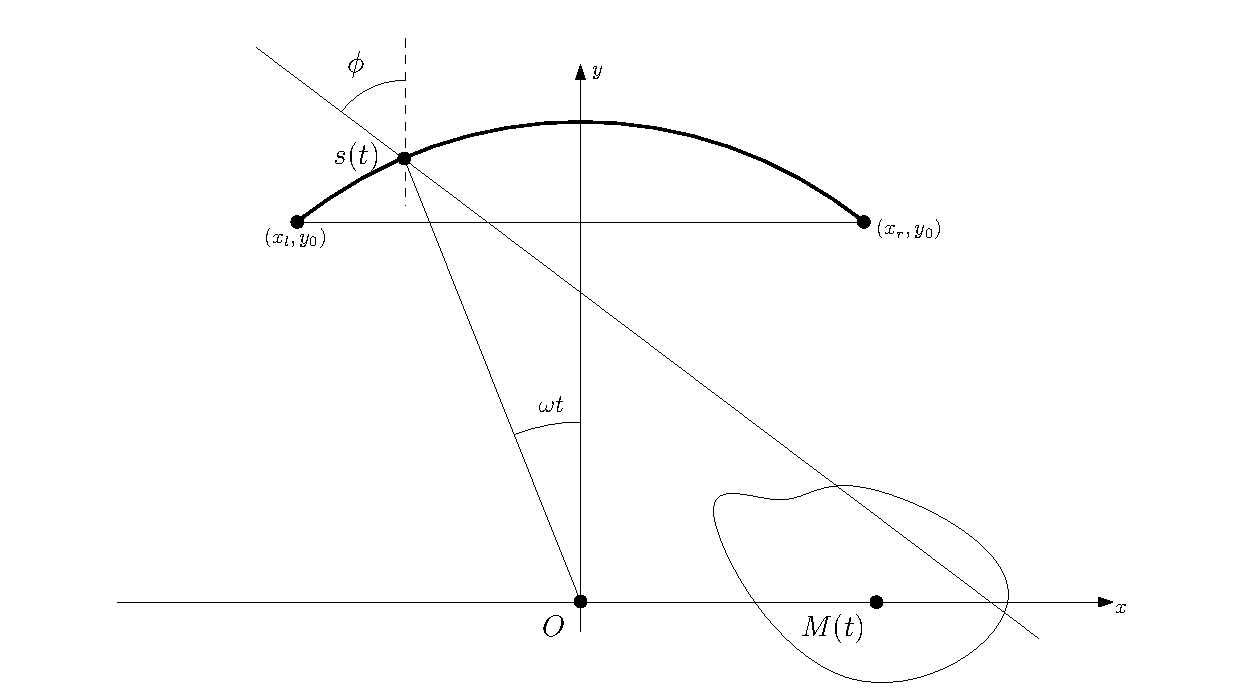
\includegraphics[width=8cm]{figs/frame_scanner.eps}
	\end{tabular}
	\caption{Problem under consideration. The source point $s(t)$ follows the arc of circle depicted in bold. This latter has center $O$ and radius $R_0$.\label{fig:notations}}
\end{figure}
The angular velocity of the source will be denoted $\omega$, and the time $t$ will range from $-T/2$ to $T/2$, where $T>0$. Hence, if we denote $s(t)$ the position of the source at time $t$, one has
\begin{equation}
	s(t) = \left( -R_0 \sin(\omega t), R_0 \cos(\omega t) \right).
\label{eq:source_position}
\end{equation}
Moreover, we will suppose that at any time $t$ rays are simultaneously emitted from the source $s(t)$ with angle $\phi$ ranging from $-\pi/2$ to $\pi/2$. With this setup in mind, we can define the operator giving the acquired data from the object.
\begin{definition}
The \emph{fanbeam projection data} of an object with density function $\mu$ is a function $(t,\phi) \mapsto T\mu(t,\phi)$ defined by
\begin{equation}
	T\mu(t,\phi) = \int_0^{+\infty} \mu \left( s(t) + l \left[ \sin \phi, -\cos \phi \right] \right) dl,
\end{equation}
where $t \in \left[ -T/2, T/2\right]$, $\phi \in \left[ -\pi/2, \pi/2\right]$ and $s(t)$ is given by~(\ref{eq:source_position}). The operator $\mu \mapsto T\mu$ is called the \emph{fanbeam projection operator}.
\end{definition}


Now let us suppose that the object is translating along the $x$-axis with a constant velocity $v \in \R$ (see Figure~\ref{fig:notations}, right). In other words, if we denote $M(t)$ its center of mass at any time $t$, we have
\begin{equation}
	M(t) =  \left( \left( t + \frac{T}{2} \right)v, 0 \right).
\label{eq:center_of_mass}
\end{equation}
In this regard, the fanbeam projection data will be modified in the following way.
\begin{definition}
The \emph{fanbeam projection data of a translating object} with density function $\mu$ and translating velocity $v$ is given by
\begin{equation}
	T_v\mu(t,\phi) = \int_0^{+\infty} \mu \left( s(t) - M(t) + l \left[ \sin \phi, -\cos \phi \right] \right) dl,
\label{eq:def_Tv}
\end{equation}
where $s(t)$ is given by~(\ref{eq:source_position}), and $M(t)$ is given by~(\ref{eq:center_of_mass}).
\end{definition}

The aim of this note is to derive data consistency conditions (DCCs) from~(\ref{eq:def_Tv}), in order to retrieve the velocity $v$.

\subsection{Derivation of DCCs}

In order to derive DCCs, we will first change our frame of reference. Indeed, let us consider Figure~\ref{fig:change_frame}, where the object is at the center.
\begin{figure}[!ht]
	\centering
	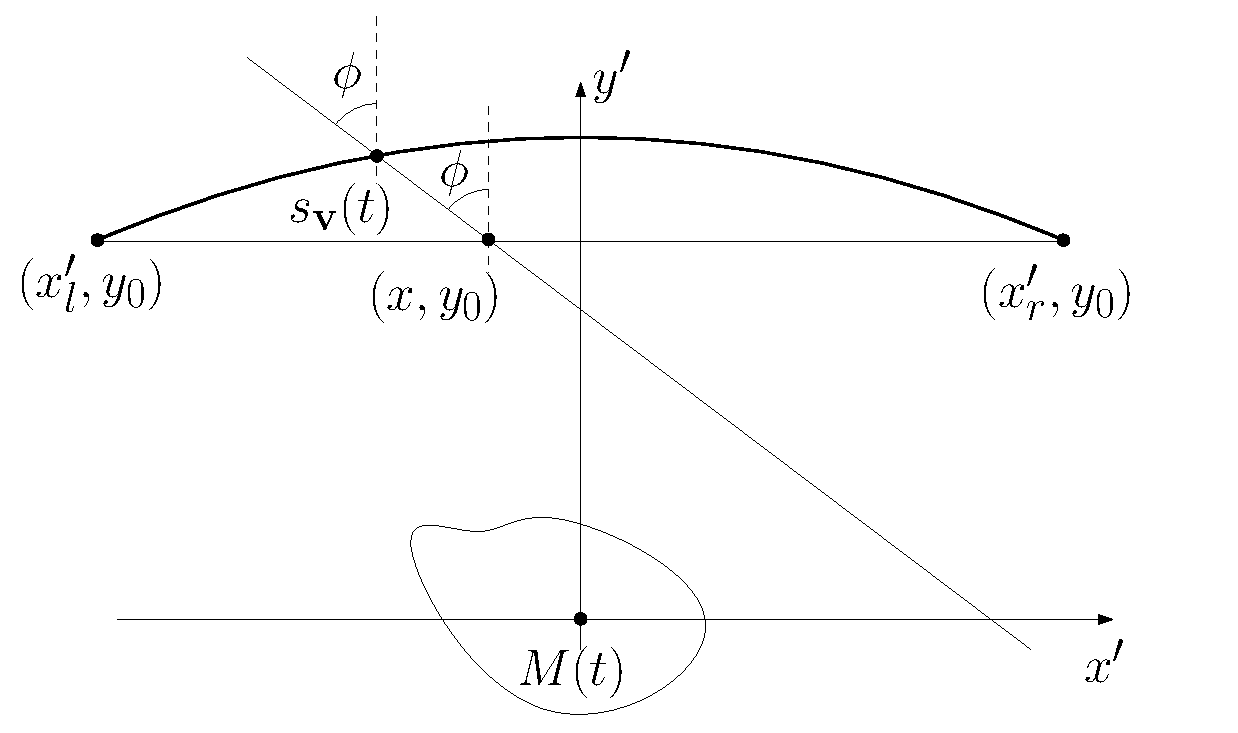
\includegraphics[width=10cm]{figs/frame_object.eps}
	\caption{Change of frame: the object is now at center of the coordinates system. The virtual point has coordinates $\left( x,y_0 \right)$\label{fig:change_frame}}.
\end{figure}
In other words, we are now dealing with a fixed object and a source following an arc of a cycloid. We will denote $R_t$ the distance between this new center and the translated source point $s_v(t)$, where the latter is given by
\begin{equation}
	s_v(t) = \left( -R_0 \sin(\omega t) - \left( t + \frac{T}{2} \right)v, R_0 \cos(\omega t) \right),
\end{equation}
with $T$ defined such that $s(-T/2) = \left(x_r,y_0\right) $ and $s(T/2) = \left(x_l,y_0\right)$. Hence, one has
\begin{equation}
R_t = \sqrt{ \left( R_0 \sin(\omega t) - \left( t + \frac{T}{2} \right)v \right)^2 + R_0^2 \cos^2(\omega t) }.	
\end{equation}
If we denote $\lambda_t$ the angle formed with the $y$-axis, we have in the same manner
\begin{equation}
\lambda_t = \arctan \left( \frac{R_0 \sin(\omega t) + \left( t + T/2 \right)v}{R_0 \cos(\omega t)} \right).
\end{equation}

The DCCs derived in~\cite{clackdoyle2015consistency} heavily rely on a relation between $\tan \phi$ and the angle $\omega t$, which is then differentiated to change variables into the following integral
\begin{equation}
	B_n(x) = \int_{-\pi/2}^{\pi/2} \tilde{g}(x,\phi) \frac{\tan^n \phi}{\cos \phi} d\phi,	
	\label{eq:Bn_x_phi}
\end{equation}
where $\tilde{g}(x,\phi)$ is the virtual fanbeam projection whose virtual source is located at $(x,y_0)$. In other words,
\begin{equation}
	\tilde{g}(x,\phi) = \int_0^{\infty} \mu\left( (x,y_0) + l(\sin \phi, -\cos \phi) \right) dl.
\end{equation}

We will follow the same path in this note. First, the formula giving $\tan \phi$ is nearly the same as in~\cite{clackdoyle2015consistency}, \emph{i.e.}
$$
\tan \phi = \frac{x + R_0 \sin(\omega t) + \left( t + \frac{T}{2} \right)v}{R_0 \cos(\omega t) - y_0}
$$
Then, taking its derivative allows us to write the Jacobian for a change of variables from $\phi$ to $t$
\begin{align*}
\frac{d\phi}{\cos^2 \phi} &= \frac{ \left( R_0 \omega \cos(\omega t) +v \right) \left( R_0 \cos(\omega t) - y_0 \right) + R_0 \omega \sin(\omega t) \left( x + R_0 \sin(\omega t) + \left( t + \frac{T}{2} \right)v \right) }{ \left( R_0 \cos(\omega t) - y_0 \right)^2 } dt \\
 &= \frac{ R_0^2 \omega - v y_0 + R_0 \cos(\omega t)(v-\omega y_0) + R_0 \omega \sin(\omega t)(x + \left( t + \frac{T}{2} \right)v ) }{ \left( R_0 \cos(\omega t) - y_0 \right)^2 } dt\\
 &:= J(x,t,v) dt.
\end{align*}
Hence, one can write
\begin{align}
	\frac{\tan^n \phi}{\cos \phi} d\phi &= \tan^n \phi \cos \phi \frac{d\phi}{\cos^2 \phi} \\
	&= \frac{ \left( x+R_0 \sin(\omega t) + \left( t + \frac{T}{2} \right)v \right)^n }{D_{x,t} \left( R_0 \cos(\omega t) - y_0 \right)^{n-1}} J(x,t,v) dt \label{eq:Dxt_first_occurence} \\
	&:= W_n(x,t,v) dt,
\end{align}
where the term $D_{x,t}$ in equation~(\ref{eq:Dxt_first_occurence}) refers to the distance between the source point $s_v(t)$ and the virtual point $(x,y_0)$.
In any case, equation~(\ref{eq:Bn_x_phi}) can be re-written as
\begin{equation}
	B_n(x,v) = \int_{-T/2}^{T/2} g(t,\phi) W_n(x,t,v) dt.
	\label{eq:Bnx_DCC}
\end{equation}

\section{Numerical simulations}

Let us suppose that we have the projections $g(x,\phi)$. In order to recover $v$, we can perform the following optimization procedure. Since $B_n(x)$ in equation~(\ref{eq:Bnx_DCC}) is supposed to be a polynom of order $\leq n$, one can minimize
\begin{equation}
	\mathcal{J}(v) = \sum_n \Vert \textrm{res} \left( B_n(x,v) \right) \Vert^2
\end{equation}
with respect to $v$, where $\textrm{res}$ is the residual of the projection onto $\R_n[X]$. The minimization procedure can be done using the gradient of $\mathcal{J}(v)$, given by
\begin{equation}
	\nabla \mathcal{J}(v) = 2 \sum_n B_n(x,v) \int_{-T/2}^{T/2} g(t,\phi) \frac{\partial W_n}{\partial v}(x,t,v) dt.
\end{equation}

\bibliographystyle{plain}
\bibliography{DCC_translation}

\end{document}

